\subsection{MQTT}
  MQTT je otevřený síťový komunikační protokol typu pulish/subcribe, který byl navržen
  v roce 1999. Již od návrhu byl zaměřen na nízkou náročnost komunikace a jednoduchost
  implementace. Díky těmto vlastnostem je velmi vhodný pro IoT a M2M systémy. \cite{mqtt}
  \subsubsection{Způsob komunikace}
  
  Protokol MQTT je postaven nad transportní vrstvou TCP (Transmission Control Protocol)
  a využívá model pulish/subcribe, který vychází z tradičního způsobu zasílání zpráv
  typu klient-server. Roli serveru zde plní speciální uzel, který se nazývá broker.
  Broker je známý všem ostatním klientům, kteří mohou zasílat zprávy pomocí operace
  publish nebo se přihlásit o příjem zpráv díky operaci subscribe.
  Na základě provedených operací broker přijímá zprávy a rozhoduje o jejich přeposlání.
  Způsob odeslání zprávy závisí na obsažených metadatech.
  
\begin{figure}[ht]
\begin{center}
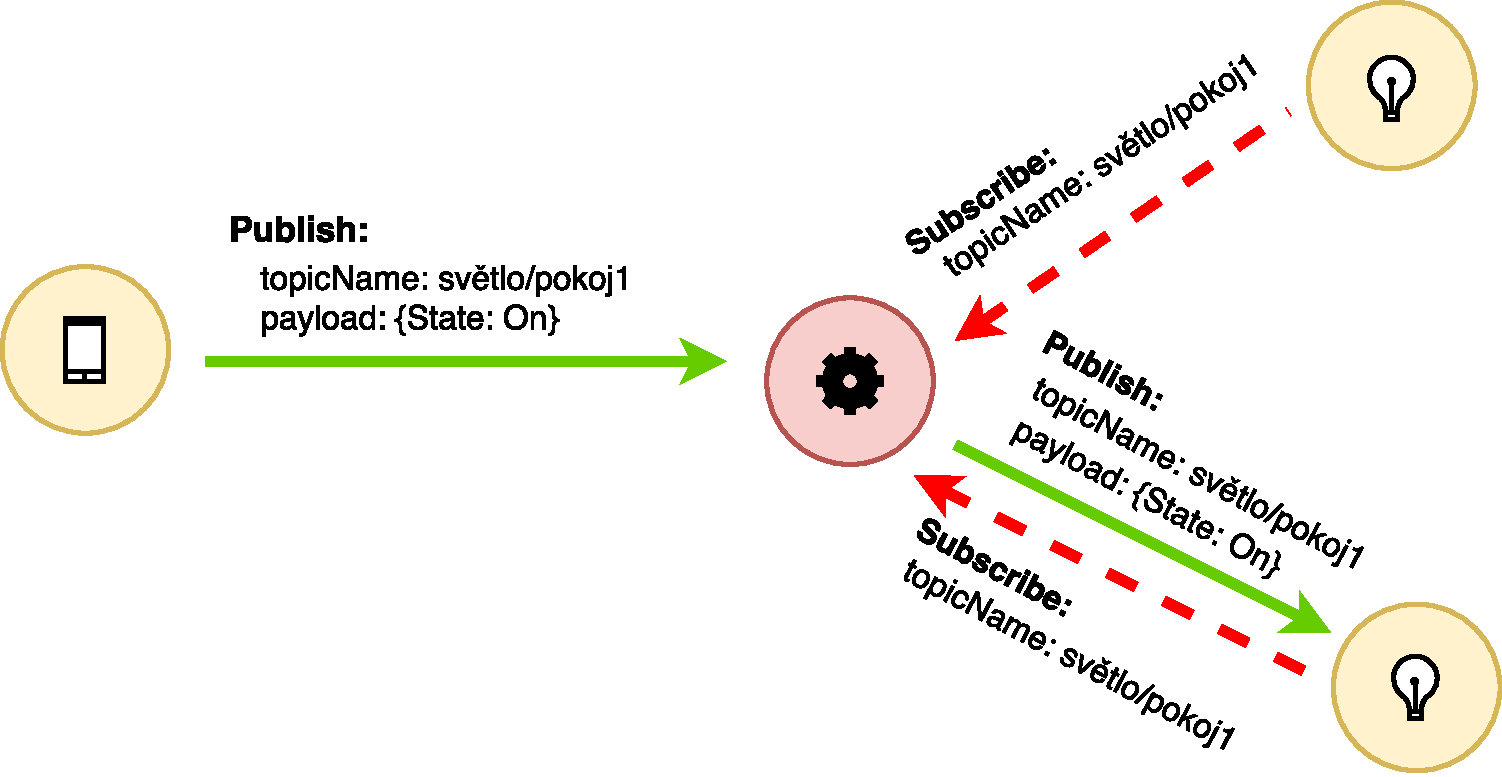
\includegraphics[scale=0.41]{pictures/mqtt-arch}
\caption{MQTT architektura}
\label{obr.mqtt-arch}
\end{center}
\end{figure}
  
  Nejčastěji o směru odesláni rozhoduje předmět (topic) zprávy. Předmět je tvořen
  jednoduchým UTF-8 řetězcem s hierarchickou strukturou, ve které jsou jednolivé
  vrstvy odděleny dopředným lomítkem (např. /domov/přízemí/světloŠatna). V předmětu
  zprávy mohou být některé vrstvy nahrazeny zástupnými symboly + a \#. Symbol + dokáže
  nahradit pouze jednu úroveň předmětu libovolným řetězcem a symbol \# umožňuje
  zastoupit více úrovní. Díky těmto symbolům mohou klienti odeslat nebo přijímat
  zprávy z více témat.
  
  Další užitečnou položkou protokolu MQTT je QoS (Quality of Service),
  která může nabývat hodnot 0, 1 nebo 2.
  
   \begin{itemize}
    \item \textbf{QoS 0}
    
    Veškeré zprávy jsou odesílány bez potvrzení a žádným způsobem
    není zvýšena úroveň spolehlivosti, která je shodná se spolehlivostí protokolu TCP.
    
    \item \textbf{QoS 1}
    
    Pomocí potvrzování zajišťuje, že každá zpráva bude příjemci doručena alespoň jednou.
    
    \item \textbf{QoS 2}
    
     Umožňuje, aby každá zpráva byla spolehlivě doručena právě jednou.
   \end{itemize}
  Hodnota QoS se nastavuje vždy mezi dvěma uzly při navazování spojení.
  Z pohledu brokeru se může stát, že přijatá a odeslaná zpráva mají jiné QoS.
  Úrovně 1 a 2 dále umožňují perzistetní ukládání zpráv v případě, že příjemce je
  nedostupný. Zároveň platí, že s vyšší úrovní roste i režie komunikace. \cite{mqtt_intro}
 \subsubsection{Bezpečnost}
 Zabezpečení protokolu MQTT je možné rozdělit do následujících vrstev:
 \begin{itemize}
  \item \textbf{Síťová vrstva}
  
    Veškerá komunikace postavena nad TCP/IP. Z tohoto důvodu je možné komunikaci
    zapouzdřit pomocí VPN (Virtual Private Network) připojení
    jako v běžných počítačových sítích. Z důvodu větších nároků na výkon je toto
    řešení vhodnější pro výkonější zařízení jako jsou například IoT brány, které
    mohou s brokerem navázat site-to-site spojení. \cite{mqtt_sec}
    
  \item \textbf{Transportní vrstva}
  
  Na této úrovni se využívá šifrování provozu pomocí protokolu TLS (Transport
  Layer Security). Omezením této metody jsou požadavky na výkon, které mohou být
  poměrně vysoké pokud nastává časté navazování spojení. \cite{mqtt_sec}
  
  \item \textbf{Aplikační vrstva}
  
  Samotný protokol MQTT nedefinuje žádné šifrovací mechanismy na aplikační úrovni. 
  Zabezpeční dat zde musí zajistit uživatel ještě před zapozdřením do MQTT zprávy. 
  Ovšem tímto způsobem je možné šifrovat jen tělo zprávy a hlavička zůstává nezměněná.
  
  Pro autentizaci je možné využít ověření pomocí jména a hesla nebo x.509 certifikátu.
  Jméno a heslo je přenášeno nešifrovaně, a proto je vhodné tuto metodu doplnit se 
  zabezpečením síťové nebo transportní vrstvy. Autentizaci pomocí certifikátů 
  je možné využít v případě použití TLS. Tato metoda je vhodnější pokud všechna
  zařízení jsou po jednotnou správou a je možné automatizovat distribuci 
  klientských certifikátů.
  
  Dále je na straně brokeru možné definovat pravidla pro autorizaci. Tyto pravidla 
  přiřazují klientů oprávnění pro provedení operací publish a subscribe
  nad příslušnými tématy. \cite{mqtt_sec}
  
 \end{itemize}

  \subsection{COAP}
  CoAP (Constrained Application Protocol) je otevřený přenosový protokol určený pro
  komunikaci síťových zařízení s velmi omezeným výkonem. Návrh vychází z RESTful
  (Representational State Transfer) principů, tudíž jeho použití je velmi vhodné
  v prostředích s již existujícím webových rozhraním, do kterého se snadno integruje. \cite{coap}
  
   \subsubsection{Způsob komunikace}
   Komunikace je postavena nad protokolem UDP (User Datagram Protocol) a vychází
   z modelu request/response, který se využívá u protokolu HTTP (Hypertext
   Transfer Protocol). Oproti protokolu HTTP je zde omezen počet možných operací
   a komunikace probíhá asynchronně. Dle důležitosti odesílané zprávy je možné určit,
   zda se má zasílat potvrzení či nikoli. Protože veškerá komunikace probíhá nad
   protokolem UDP, tak přenášené zprávy obsahují položku Message ID, která dokáže
   ošetřit duplikaci přijatých dat.
   %pokud to bude krátků můžu přidat option políčka pro udělání akce po splnění podmíky
   
   Pro zajištění integrace s běžnými webovými službami a zachování nízkých nároků
   se v CoAP topologii velmi často vyskytují proxy servery. Tyto servery mohou plnit
   funkci běžných reverzních a dopředných proxy, mapování mezi CoAP a HTTP protokolem
   nebo vyvažování zátěže. 
   
   \begin{figure}[ht]
   \begin{center}
   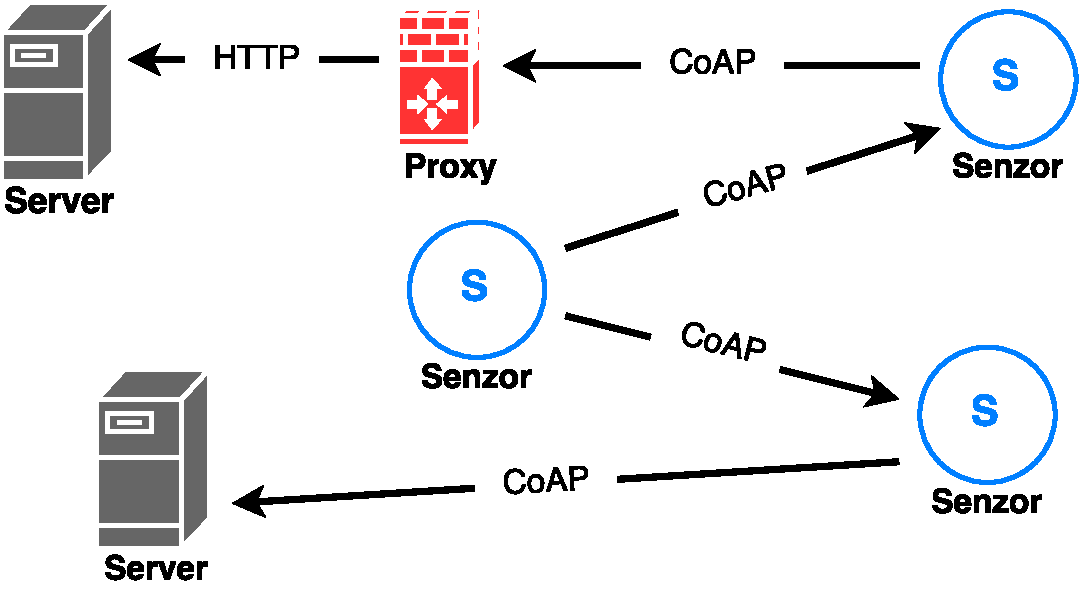
\includegraphics[scale=0.41]{pictures/coap-arch}
   \caption{COAP architektura}
   \label{obr.coap-arch}
   \end{center}
   \end{figure}
   
   Ve specfikaci protokolu CoAP jsou definovány následující operace:
   \begin{itemize}
    \item \textbf{GET}
    
    Metoda \textit{GET} vrací aktuální stav požadovaného zdroje, který je identifikován pomocí
    URI (Uniform resource identifier). Tato operace je vždy bezpečná a idempotentní.
    
    \item \textbf{POST}
    
    \textit{POST} požadavek obsahuje ve svém těle novou reprezentaci cílového zdroje a požaduje 
    jeho zpracování. Funkce, která
    novou reprezentaci přijímá je definovaná na cílovém uzlu s příslušným URI.
    Výsledkem je vytvoření nového zdroje nebo aktualizace původního. Tato metoda
    není z pohledu zpracování bezpečná ani idempotentní.
    
    \item \textbf{PUT}
    
    Tato metoda specifikuje nový stav cílového zdroje, který se buď vytvoří, nebo 
    v případě jeho existence aktualizuje. Provedení operace není bezpečné, ale 
    je idempotentní.
    
    \item \textbf{DELETE}
    
    Operace \textit{DELETE} požaduje smazání zdroje s příslušným URI. Tato metoda není bezpečná,
    ale je idempotentní.
    
   \end{itemize}
   
   Vyhledání potřebného zdroje je v topologii protokolu CoAP možné provést pomocí
   znalosti jeho URI nebo odesláním multicastového požadavku na definovanou
   skupinu uzlů. Možnost vyhledávání cílových zdrojů je velmi důležitá zejména
   v M2M prostředích. \cite{coap}
   
   \subsubsection{Bezpečnost}
   Samotný protokol nijak nedefinuje možnost autentizace a autorizace. V případě
   potřeby je nutné tyto mechanismy implementovat v aplikačním kódu. 
   
   Pro zajištění šifrování provozu nabízí CoAP následující režimy:
   \begin{itemize}
    \item \textbf{NoSec}
    
    Tento mód neobsahuje žádnou úroveň zabezpeční a veškeré zprávy jsou zasílány
    v otevřené podobě. 
    
    \item \textbf{PreSharedKey}
    
    V tomto případě se náváže spojení pomocí protokolu DTLS (Datagram Transport
    Layer Security), které využívá symetrické šifrování. Předsdílený klíč musí
    být známý všem uzlům před zahájením komunikace. 
    
    \item \textbf{RawPublicKey}
    
    Tento režim také navuzuje zabezpečené spojení pomocí protokolu DTLS, ale místo
    symetrické šifry se používá asymetrická.
    
    \item \textbf{Certificate}
    
    Mód \textit{Certificate} rozšiřuje \textit{RawPublicKey} o přidání certifikátu.
   \end{itemize}

   Podobně jako u protokolu MQTT je i zde možné ochránit provoz na síťové
   vrstvě pomocí VPN. Při nasazení libovolného režimu zabezpeční je nutné počítat 
   s většími nároky na výkon, které musí klient splňovat pro navazování a udržování 
   spojení. \cite{coap}
   
  \subsection{Z-Wave}
  
  Z-Wave je bezdrátový komunikační protokol určený pro senzorové sítě, který vysílá 
  v subgigahercových pásmech ISM (Industrial, Scientific and Medical). Veškeré komunikační
  prvky jsou certifikovány aliancí Z-Wave, která zároveň poskytuje technickou dokumentaci a
  licence pro vývoj. V současné době existují certifikace Z-Wave a Z-Wave Plus. 
  Z-Wave Plus zařízení obsahují nový chipset, který vylepšuje komunikační parametry
  sítě a zároveň je zpětně kompatibilní se staršími modely. \cite{z-plus}
  Otevřená implementace celého protokolu se nazývá OpenZWave \cite{openzwave}, která
  je vyvíjena komunitou. \cite{cesnet-survey} 
 
 \subsubsection{Způsob komunikace}
 V Z-Wave síti se může maximálně vyskytovat 232 uzlů, mezi kterými se vždy nachází jeden označený
 jako kontroler. Pro přidání libovolného zařízení do sítě musí být nejprve provedo příme spárování
 s kontrolerem. Během párovacího procesu nový prvek získá vlastní 8 bitový identifikátor (\textit{Node ID}) a 
 unikátní 32 bitový identifikátor sítě (\textit{Home ID}), který má již od výroby kontroler uložen v nepřepisovatelné paměti.
 Následné zasílání zpráv už nemusí probíhat přímo mezi senzorem a kontrolerem, ale zprávy mohou
 být přeposílány sousední prvky, které jsou trvale napájené, čímž se velmi zvyšuje možná rozloha sítě. 
 Pro odebrání libolného zařízení je opět nutné zajisiti přimé spojení s kontrolerem a spustit odstraňovací
 proces. \cite{cesnet-survey}
 
 V rámci specifikace Z-Wave \cite{zwave-spec} je definován mechanismus pro určení dostupných příkazů. Každý senzor obsahuje
 svou definici tříd funkcionalit (\textit{Command Class}), které obsahují dostupné příkazy a formát odpovědi. Tyto definice
 jsou předány kontroleru během procesu párování. Příkladem může být třída \textit{Binary Switch}, která obsahuje příkazy:
 \begin{itemize}
 \item \textit{SET} - odesílá kontroler pro nastavení hodnoty 
 \item \textit{GET} - odesílá kontroler pro získání hodnoty  
 \item \textit{REPORT} - odesílá senzor jako odpověď na dotaz \textit{GET} 
 \end{itemize} 
 
 Při posílání zpráv je vždy vyžadováno potvrzení. V případě neobdržení potvrzení se vysílání opakuje. 
 Po třetím neúspěšném pokusu je požadavek zahozen.
 
 \subsubsection{Bezpečnost}
 Původní verze protokolu Z-Wave umožňovala volitelně využívat šifrování pomocí 128 bitového AES (Advanced Encryption Standard).
 Výměna symetrického klíče probíhá během počátečního párování, kde je vygenerovaný klíč šifrován pomocí výchozího
 klíče, který je uložen ve firmwaru. Vzhledem k tomuto postupu je dobré provádět počáteční párování na bezpečném
 místě, kde nemůže dojít k odposlechu. \cite{zwave-S0-attack}
 
 V roce 2016 Z-Wave aliance vydala nový S2 (Security 2) framework, který vylepšuje bezpečnostní funkcionality 
 a od roku 2017 je jeho použití povinné pro všechny nově certifikovaná zarízení. 
 
 S2 framework umožňuje zařízení rozdělit do následujících skupin s rozdílnými šifrovacími klíči:
 \begin{itemize}
  \item \textbf{Access Control} - 
   nejdůvěryhodnější třída, která obsahuje bezpečnostní prvky jako jsou například zámky,
   které zároveň podporují autentizaci
  \item \textbf{Authenticated} - 
  skupina určená pro běžné senzory, které podporují autentizaci 
  \item \textbf{Unauthenticated} - 
  třída pro ostatní prvky, které nepodporují autentizaci.
 \end{itemize}
 Autentizace probíhá pomocí PIN (Personal Identification Number) nebo QR (Quick Response) kódu.
 Výměna klíče je založena na algortmu ECDH (Elliptic-curve Diffie–Hellman), který zajišťuje 
 dostatečnou úroveň bezpečnosti během párovacího procesu. \cite{cesnet-survey}

 
  \subsection{BLE (Bluetooth Low Energy)}
  BLE je bezdrátový prtokol určený pro senzorové sítě s důrazem na nízkou spotřebu. Byl představen 
  v roce 2010 jako součást specifikace Bluetooth 4.0 a je nekompatibilní s původními verzemi. 
  Za vývoj a údržbu protokolu je odpovědná skupina Bluetooth SIG (Special Interest Group).
  V současné době je nejnovější verzí Bluetooth 5.
  
  \subsubsection{Způsob komunikace}
  BLE vysílá v bezlicenčním ISM pásmu na frekvencích od 2.4 GHz do 2.4835 GHz. Specifikace
  protokolu vychází z Bluetooth, ale zejména díky změnám parametrů v rádiové vrstvě 
  jsou navzájem nekompatibilní. Do verze 4 umožňuje navázat pro koncová zařízení pouze jedno spojení a 
  vytváří tak hvězdicovou topologii s jedním centrálním prvkem. Od verze 5 je možné využívat více připojení
  a vytvořit tak flexibilnější mesh topologii. 
  
  Před zahájením komunikace mezi centrálním prvkem a senzory je nutné nejprve prvést párování, 
  které probíhá v následujících krocích:
  \begin{itemize}
   \item \textbf{Vysílání žádostí}
   
   Při spuštění párování začně koncový prvek na kanálech určených pro propagaci všesměrově vysílat žádosti o připojení,
   které obsahují název zařízení, jméno výrobce a podporované služby.
   
   \item \textbf{Přijímání žádostí}
   
   Pokud je centrální prvek přepnutý do párovacího režimu, tak naslouchá příchozím požadavkům, které zobrazuje uživateli.
   Po výběru správného zařízení se ukončí mód naslouchání a začne se navazovat spojení.
   
   \item \textbf{Inicializace připojení} 
   
   Během této fáze se obě strany domlouvají na parametrech komunikace.
   \item \textbf{Komunikace}
   
   Po úspěšném navázání spojení je možná na základě dostupných služeb provádět zasílání zpráv.
  \end{itemize}

 
   \subsubsection{Bezpečnost}
   BLE umožňuje volitelně používat šifrování pomocí AES, jehož šifrovací klíč je 
   vytvořen behěm párování v části inicializace připojení. Velmi důležité je zabezpečit 
   výměnu sdíleného klíče, která až do verze 4.1 není bezpečná, protože neumožňuje ochranu
   před odposloucháváním. Vylepšení přichází až od verze 4.2, ve které lze využít ECDH.
   
   Vzhledem k různorodosti možných typů zařízení definuje BLE následující kategorie
   určující způsob výměny klíče:
    \begin{itemize}
     \item \textbf{Just Works}
     
     Nejjednodušší třída, která provádí výměnu automaticky a zároveň má nejmenší nároky 
     na připojované zařízení, které nemusí podporovat autentizaci. Díky chybějící autentizaci 
     je tato metoda zranitelná vůči MITM (Man in the middle) útokům.
     \item \textbf{Out of Band}
     
     V této kategorii jsou veškeré klíče vyměňovány odlišným komunikačním kanálem např. přes NFC (Near Field Communication).
     Celková bezpečnost této metody závisí na důvěryhodnoti použitého kanálu.
     \item \textbf{Passkey}
     
     Tato metoda vylepšuje \textit{Just Works} o autentizaci, která spočívá v uživatelském zadání šesti 
     místného kódu. Pro ochranu před odposlouchávání musí být použit algoritmus ECDH, který je dostupný
     až od verze 4.2.
     
     \item \textbf{Numeric Comparison}
     
     Využití tohoto způsobu párování je možné pouze od verze 4.2. Dochází zde k rozšíření metody \textit{Just Works}
     o jeden kontrolní krok, který slouží jako ochrana před MITM útokem. Po výměně klíčů každé zařízení
     vygeneruje šestimístný číselný kód, který následně zobrazí uživateli a čeká na jeho potvrzení.   
     
    \end{itemize}
